\subsection{Uzyskane wartości wyrazów ciągu}

\quad Najpierw opiszemy wyniki uzyskane dla float32 i $n = 225$.
\begin{figure}[h!]
	\centering{
		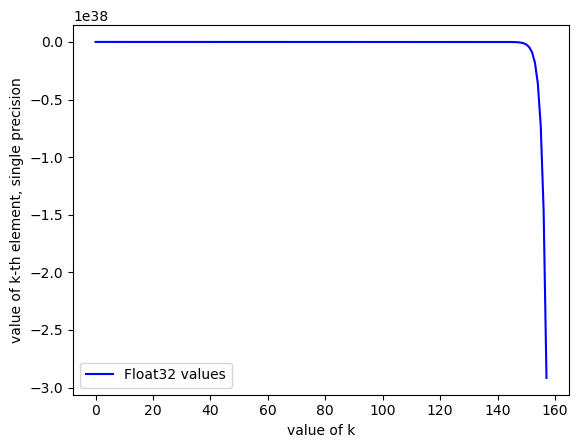
\includegraphics[width=0.67\textwidth]{img/float32-1.png}
	}
	\caption{Nieskalowany wykres wartości ciągu dla float32}
	\label{zad2:graph1}
\end{figure}
Widzimy, że po pewnym wyrazie ciągu (dokładniej po 9.), wszystkie wartości schodzą poniżej 0 i~ciąg jest stale malejący. Wyjaśnić to można poprzez zjawisko zwane 
\emph{underflow}~\cite{underflow_wiki}. W~pewnym momencie brakuje dokładności reprezentacji float32, żeby wystarczająco dokładnie zapisać wynik danego obliczenia i~wartość jest zaokrąglona 
do najbliższej możliwej - w tym przypadku okazuje się, że w~pewnym momencie jest nią liczba mniejsza od 0 w~reprezentacji float32.
\newline
\textbf{Uwaga!} Dla $k > 157$ wartości są tak małe, że wynik obliczenia jest nieokreślony ($-\infty$, dla $k > 159$ jest to nan). Zatem na powyższym wykresie nie są one obecne.

\newpage
Dla porównania przedstawiamy wykres, gdy nie używamy funkcji \emph{np.float32} na współczynnikach ciągu i~dostajemy bardziej sensowny, przypominający float64 wykres.
\begin{figure}[ht!]
	\centering{
		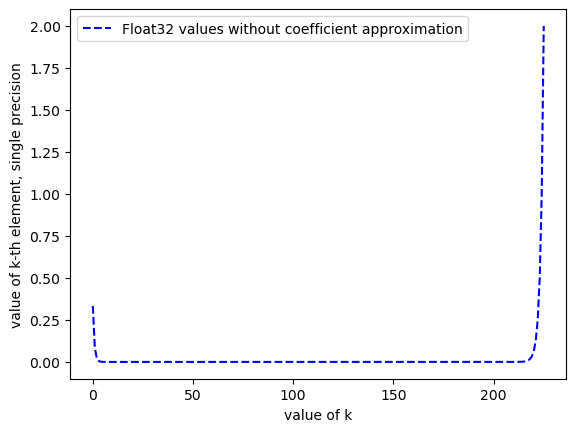
\includegraphics[width=0.67\textwidth]{img/float32-coeff.png}
	}
	\caption{Nieskalowany wykres wartości ciągu dla float32 bez przybliżenia współczynników}
	\label{zad2:graph2}
\end{figure}

Moglibyśmy wykorzystać ten sposób do obliczenia wyrazów ciągu, ale wtedy okazuje się, że float32 jest bardziej dokładny od float64 (w~dalszych testach błędu względnego float32 miałoby mniejszy błąd). Uznajemy to za niezbyt sensowne i~postanowiliśmy testować wszystkie funkcje, wykorzystując przybliżenie współczynników ciągu - nie patrzymy na to, że float32 ucieka do~$-\infty$, a~float64 do~$+\infty$. 

Poniżej przedstawiony jest wykres logarytmiczny wartości bezwzględnej wyrazów ciągu w~reprezentacji float32 (wykorzystujemy wartość bezwzględną dla wygody porównania wykresów z~ciągiem float64 w~przyszłości).
\begin{figure}[ht!]
	\centering{
		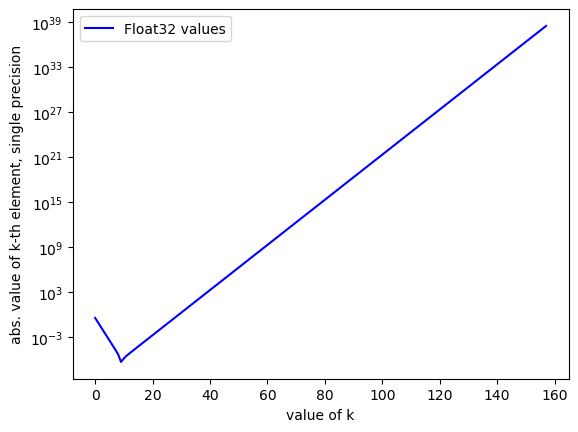
\includegraphics[width=0.67\textwidth]{img/float32-2.png}
	}
	\caption{Wykres symlog wartości ciągu dla float32}
	\label{zad2:graph3}
\end{figure}

\newpage
Poniżej prezentujemy logarytmiczny wykres wartości ciągu dla reprezentacji float64. 
\begin{figure}[ht!]
	\centering{
		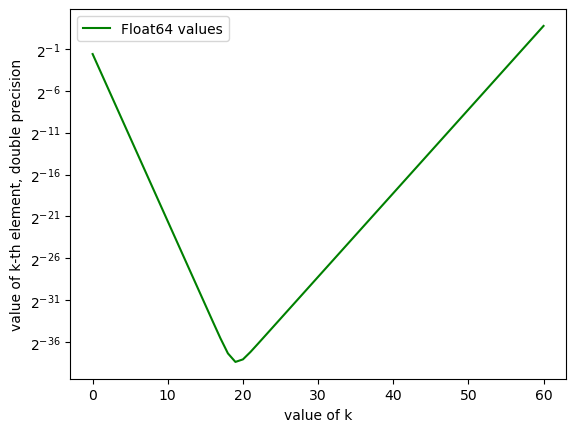
\includegraphics[width=0.67\textwidth]{img/float64.png}
	}
	\caption{Logarytmiczny wykres wartości ciągu dla float64}
	\label{zad2:graph4}
\end{figure}

Jak widać, podobnie do float32 (w~drugim rozważanym przypadku), float64 w~pewnym momencie osiąga minimum i~zaczyna rosnąć. Znowu związane to jest z~tym, że w~pewnym momencie 
następuje underflow, brakuje precyzji reprezentacji float64, żeby dokładnie przedstawić liczbę i~wykorzystywane są przybliżenia. Z~czasem coraz większa ilość przybliżeń się sumuje i~dostajemy wyrazy coraz bardziej różniące się od 
wartości rzeczywistej. W~pewnym momencie błąd reprezentacji powoduje, że wartość $x_k$ jest większa od $x_{k-1}$ i~wtedy ciąg rośnie w~nieskończoność.
\newline
\newline
Teraz spójrzmy na wykres dla reprezentacji z~biblioteki fractions.
\begin{figure}[ht!]
	\centering{
		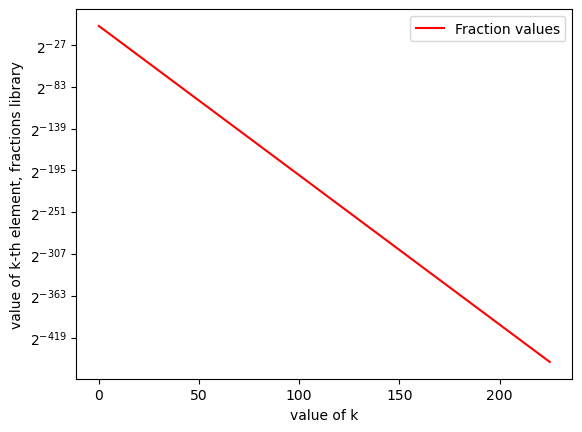
\includegraphics[width=0.67\textwidth]{img/fractions.png}
	}
	\caption{Logarytmiczny wykres wartości ciągu dla fractions}
	\label{zad2:graph5}
\end{figure}

Widać, że to jest najbardziej dokładna prezentacja. Ciąg wartości jest malejący i~większy od zera oraz reprezentuje dokładnie wartości wyliczone z~postaci jawnej ciągu (zobaczymy to poniżej, przy opracowaniu błędów względnych). Prawdopodobnie związane to jest z~tym, że postać jawna ciągu to 
$x_k = \frac{4^{-k}}{3}$, czyli każdy wyraz ciągu da się przedstawić dokładnie w~postaci ułamka i~patrząc na to, co Fractions robi pod spodem (mnoży, ewentualnie dodaje mianowniki i~liczniki, a~potem skraca ułamek), to taką dokładność można łatwo uzasadnić tym, że w~każdym momencie działamy na liczbach całkowitych (mianowniku i~liczniku). Dla naszego przypadku, kiedy wyrazy ciągu są wymierne i~w~dodatku do tego łatwo znaleźć k-ty wyraz w~postaci ułamka, Fraction jest najbardziej sensowną reprezentacją.

Poniżej przedstawiamy porównanie wszystkich wyników. Zauważamy między innymi, że rzeczywiste wartości ciągu w~zasadzie nakładają się na wykres wartości uzyskanych z~Fraction.
\begin{figure}[ht!]
	\centering{
		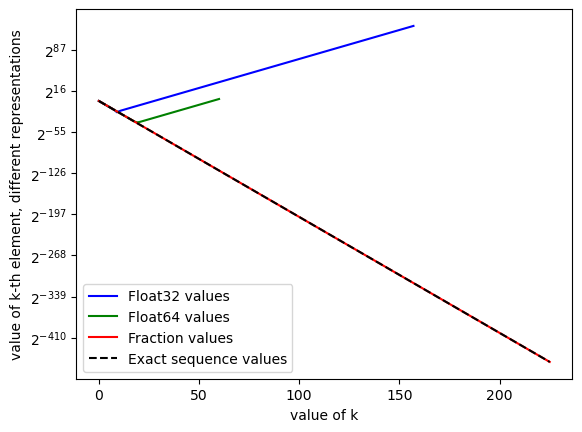
\includegraphics[width=0.67\textwidth]{img/all-values.png}
	}
	\caption{Wykres wspólny wartości ciągu dla różnych precyzji}
	\label{zad2:graph6}
\end{figure}

\subsection{Błędy względne}
\quad Przechodząc teraz do opracowania błędów względnych naszych reprezentacji, zaczniemy znów od float32.
\begin{figure}[h!]
	\centering{
		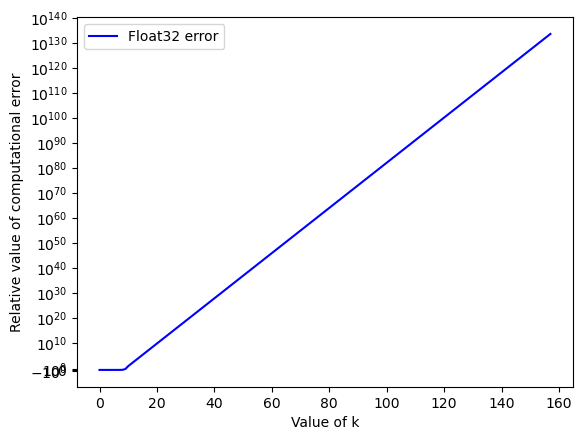
\includegraphics[width=0.67\textwidth]{img/float32-err.png}
	}
	\caption{Logarytmiczny wykres błędu względnego wyrazów ciągu dla float32}
	\label{zad2:graph7}
\end{figure}

Tak jak przewidywaliśmy przy wyjaśnieniu zachowania wykresów float32 i~float64, do pewnego momentu obliczenia są zapisywane w~miarę dokładnie, ale po jakimś czasie ograniczona precyzja powoduje underflow i~błąd zaczyna rosnąć eksponencjalnie (wykres jest w~skali logarytmicznej). Można zatem stwierdzić, że reprezentacja float32 dla naszego ciągu była dokładna tylko dla pierwszych 10 wyrazów.

Podobną analizę przeprowadzamy dla reprezentacji float64.
\begin{figure}[h!]
	\centering{
		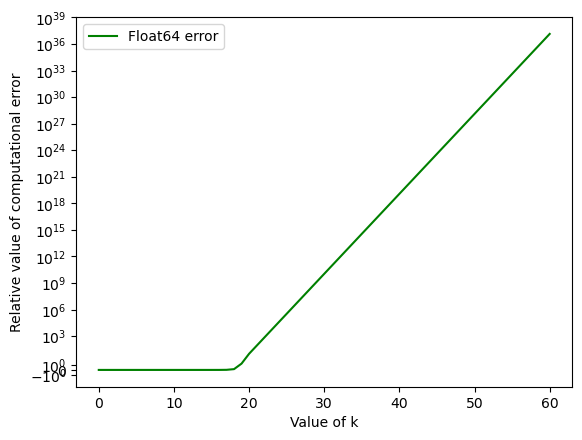
\includegraphics[width=0.67\textwidth]{img/float64-err.png}
	}
	\caption{Logarytmiczny wykres błędu względnego wyrazów ciągu dla float64}
	\label{zad2:graph8}
\end{figure}

Widzimy podobną do float32 sytuację - do pewnego momentu nasze obliczenia mają dużą precyzję, ale po tym, jak dochodzimy do momentu, gdy wiele underflow z rzędu powoduje zmniejszenie precyzji, błąd rośnie bardzo szybko.

Fractions wyróżnia się spośród badanych reprezentacji swoim zerowym błędem.
\begin{figure}[h!]
	\centering{
		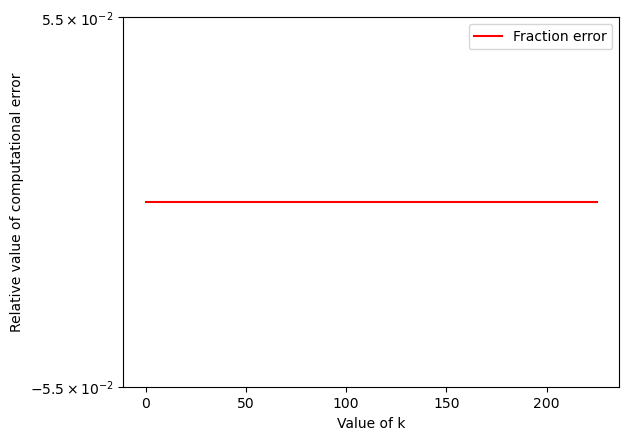
\includegraphics[width=0.67\textwidth]{img/fractions-err.png}
	}
	\caption{Logarytmiczny wykres błędu względnego wyrazów ciągu dla fractions}
	\label{zad2:graph9}
\end{figure}

Ponownie nasze spostrzeżenia odnośnie dobrej precyzji fractions w tym zadaniu (między innymi ze względu na to, że wyraz ogólny ciągu da się w~prosty sposób opisać za pomocą odpowiedniego ułamka) się sprawdzają. 

\newpage
Podsumujmy nasze rozważania, przedstawiając wspólny wykres wszystkich błędów względnych.
\begin{figure}[h!]
	\centering{
		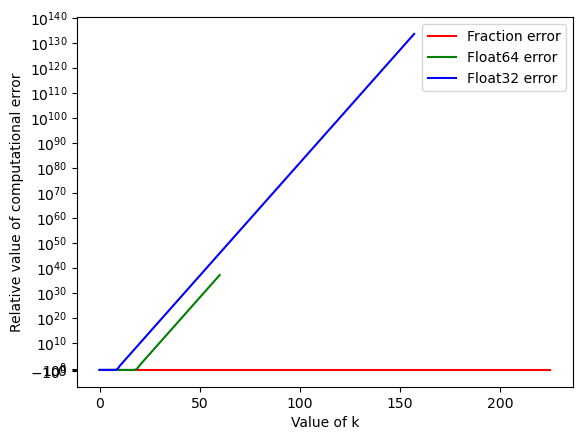
\includegraphics[width=0.67\textwidth]{img/all-err.png}
	}
	\caption{Logarytmiczny wykres błędu względnego wyrazów ciągu dla wszystkich precyzji}
	\label{zad2:graph10}
\end{figure}

Na tym wykresie widzimy, na ile floaty zachowują się w~podobny sposób. Poniżej na kolejnym wykresie lepiej widać 
moment, gdy każdy z~floatów zaczyna szybko tracić precyzję.

\begin{figure}[h!]
	\centering{
		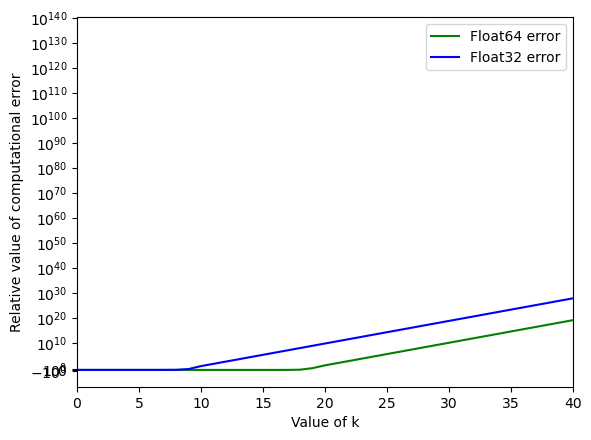
\includegraphics[width=0.67\textwidth]{img/float64-32-err.png}
	}
	\caption{Porównanie wartości błędu względnego dla float32 i~float64}
	\label{zad2:graph11}
\end{figure}

Z opracowania danych wynika, że float32 osiąga swoje minimum dla 9. wyrazu, a float64 dla 19. wyrazu. To jest mniej więcej zgodne z~przedstawieniem tego, jaką precyzję ma każda z~tych reprezentacji, gdyż float64 używa dwa razy więcej bitów i~wartość minimalna jest rzędu $10^{-12}$, a~w~przypadku float32 jest to tylko $10^{-7}$ (dla porównania, najmniejszy wyraz ciągu obliczonego za pomocą fractions to około $10^{-136}$). Ciekawym i~może trochę kontrintuicyjnym spostrzeżeniem jest to, że zarówno błędy względne float32, jak i~float64, mają podobne tempo wzrostu po momencie, kiedy zaczynają gwałtownie rosnąć.

\newpage  
